\documentclass[12pt]{article}

\usepackage[fontset=none]{ctex}
\setCJKmainfont{Noto Serif CJK SC}
\setCJKsansfont{Noto Serif CJK SC}
\setCJKmonofont{Noto Sans CJK SC}

\usepackage{graphicx,float,indentfirst,amsmath,amssymb,geometry,subfig,hyperref}

\hypersetup{hidelinks}

\geometry{a4paper,scale=0.8}

\title{电磁感应报告}
\author{}
\date{\today}

\begin{document}

\maketitle
\setlength{\parindent}{2em}

\section*{摘要}
本实验欲对线圈的自感/互感的相关参量及规律进行测量研究。通过对含电感电路的相关的参数的测量,计算了指定电感线圈在有铝芯和无铝芯情况下的电阻和电感。并通过搭建互感电路,测定了互感系数和次级线圈的反射等参量。并进一步探究了它们之间的关系。最后,对涡流进行了简单的分析。

\section{线圈电阻和电感及互感系数}

\subsection*{原理}
为测量感抗和电阻,我们对线圈串联一个已知电阻以获得电流。根据电磁感应的知识,可推出线圈电阻的表达式:
\begin{equation}
    R = \frac{R'}{2}(\frac{V_A^2-V^2}{V_{R'}^2}-1)
    \label{eq:1}
\end{equation}
其中,$R'$与$V_{R'}$表示已知电阻及两端电压,$V_A$为输出电压,$V$为线圈两端电压。同时,可根据下式计算出阻抗$Z$及感抗$X$:
\begin{equation}
    \begin{split}
        &Z = \frac{V}{V_{R'}}R' \\
        &X = \sqrt{Z^2-R^2}
    \end{split}
    \label{eq:2}
\end{equation}
而电感$L=\frac{X}{\omega}$,已知频率,便可得出电感。在次级线圈处,测出电压$V_O$,根据:
\begin{equation}
    \omega M I_P = I_S Z_S
    \label{eq:3}
\end{equation}
(其中P-初级线圈,S-次级线圈)根据电压和所计算的电阻,感抗,即可得到互感系数$M$。

\subsection*{实验步骤及数据处理}
在此部分以及下面的各部分中,我们将电源(信号发生器)调整为1000Hz,7V有效值的正弦波输出。按照原理部分搭建电路,最终通过所测得数据即可计算出电阻,电感以及互感系数。(为测量精准,我们通过调整电阻,人为保证$V \approx V_{R'}$)

测量数据如表\ref{tab:A1},而计算结果如下:
\begin{table}[H]
    \centering
    \begin{tabular}{|l|c|c|c|c|}
    \hline
           & $R(\Omega)$ & $Z(\Omega)$ & $X(\Omega)$ & $L(H)$ \\ \hline
    线圈1无铝芯 & 52.50       & 574.5       & 572.1       & 0.572  \\ \hline
    线圈2无铝芯 & 54.62       & 623.0       & 620.6       & 0.621  \\ \hline
    线圈1+铝芯 & 86.72       & 477.0       & 469.1       & 0.469  \\ \hline
    线圈2+铝芯 & 129.8       & 411.2       & 390.2       & 0.390  \\ \hline
    \end{tabular}
    \caption{线圈的电阻,阻抗,电感}
    \label{tab:1}
\end{table}
进一步,根据上述表格,求出$I_P$,$I_S$,进一步求出M,如下表:
\begin{table}[H]
    \centering
    \begin{tabular}{|l|c|c|c|}
    \hline
    数据来源   & $I_P(mA)$ & $I_S(mA)$ & $M(H)$ \\ \hline
    线圈1无铝芯 & 8.057     & 6.157     & 0.4761 \\ \hline
    线圈1+铝芯 & 9.196     & 7.295     & 0.3262 \\ \hline
    \end{tabular}
    \caption{线圈的互感系数}
    \label{tab:2}
\end{table}

由于耦合线圈的互感和自感之间的关系为$M=k(L_1L_2)^{\frac{1}{2}}$,可求出,无铝芯耦合常数$k=0.799$,有铝芯时$k=0.763$。

\section{互感与次级线圈感抗}

\subsection*{原理}
还有一种方法可以获得互感与次级线圈感抗,根据\ref{eq:3}式,将\ref{eq:2}式带入,可获得:
\begin{equation}
    (R_s+R_L)^2=\omega^2 M^2 (\frac{I_P}{I_S})^2 - X_s^2
    \label{eq:4}
\end{equation}
这是一条直线,故可通过调整$R_L$(负载)获得多组值,从而进行直线拟合以求出互感$M$与次级线圈感抗$X_S$。

\subsection*{实验步骤及数据处理}
取出铝芯,如下图搭建电路,其中$R'=300\Omega$,$R_L$可调,从$100\Omega$到$1000\Omega$间隔$100\Omega$,共10组数据。
\begin{figure}[H]
    \centering
    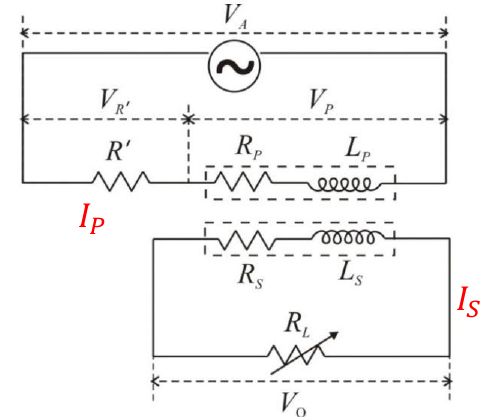
\includegraphics[width=0.5\textwidth]{fig_circuit.png}
    \caption{电路图}
    \label{fig:1}
\end{figure}
电源输出不变,不断按上面所述调整$R'$,得到的数据见\ref{tab:A2},通过对应电阻求出$I_P$,$I_S$,根据\ref{eq:2}式求出$X_S$,根据\ref{eq:4}式对相应数据进行拟合,结果如图:
\begin{figure}[H]
    \centering
    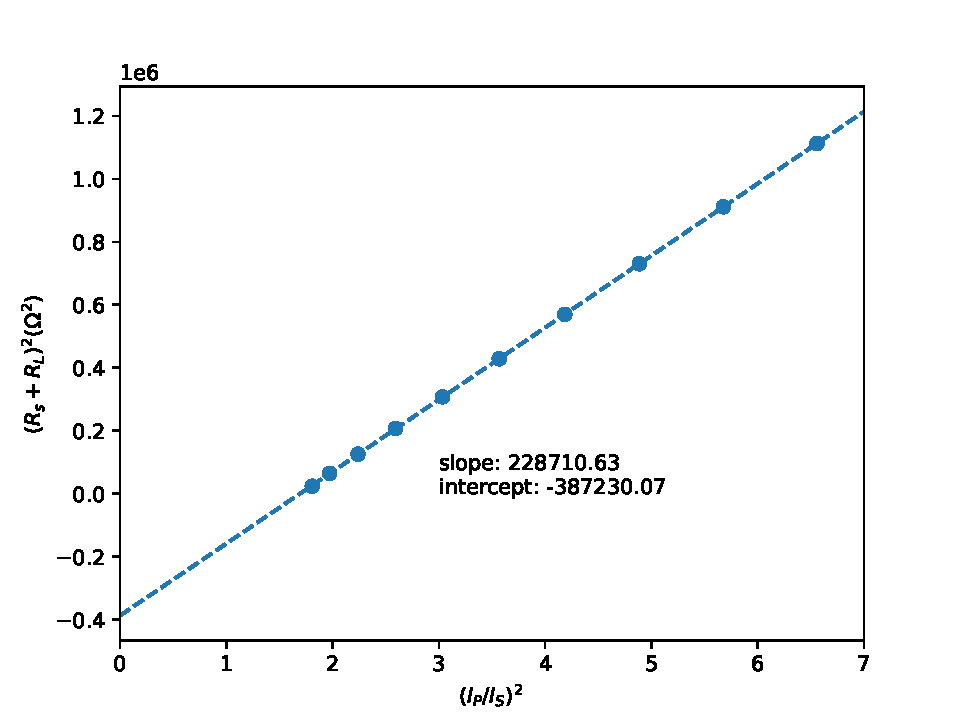
\includegraphics[width=0.7\textwidth]{fig_opt1.pdf}
    \caption{互感与次级线圈感抗拟合结果}
    \label{fig:2}
\end{figure}
对应的$\omega^2 M^2 = 228710.63$,即$M = 0.4782H$,对比\ref{tab:2},无铝芯情况下$M = 0.4761H$,相差仅0.44\%,精度很高。

对应的$X_S^2 = 387230.07$,$X_S=622.3\Omega$,对比\ref{tab:1},无铝芯下,线圈二$X_S=620.6\Omega$,相差仅0.27\%,仍然精度很高。

\section{初级线圈的等效阻抗和次级线圈的若干反射物理量之间的关系}
\subsection*{原理}
初级线圈的等效电阻$R_{PE}$和等效电感$L_{PE}$与来自于次级线圈的“反射”电阻$R_{R}$和“反射”电感$L_R$有关。反射电阻与反射电感满足:
\begin{equation}
    I_P^2R_R=I_S^2(R_S+R_L)
    \label{eq:5}
\end{equation}
\begin{equation}
    \frac{1}{2}L_RI_P^2=\frac{1}{2}L_SI_S^2
    \label{eq:6}
\end{equation}

\subsection*{实验步骤及数据处理}
对\ref{fig:1}的上半部分电路使用第一部分的方法(式\ref{eq:1}、\ref{eq:2})即可得到初级线圈等效电阻$R_{PE}$和等效感抗$X_{PE}$,如下表:
\begin{table}[H]
    \centering
    \begin{tabular}{|c|c|l|}
    \hline
    \multicolumn{1}{|l|}{$R_L(\Omega)$} & \multicolumn{1}{l|}{$R_{PE}(\Omega)$} & $X_{PE}(\Omega)$ \\ \hline
    100                                 & 135.6                                 & 228.7            \\ \hline
    200                                 & 179.1                                 & 259.4            \\ \hline
    300                                 & 209.0                                 & 296.1            \\ \hline
    400                                 & 226.3                                 & 333.6            \\ \hline
    500                                 & 233.7                                 & 368.6            \\ \hline
    600                                 & 234.9                                 & 398.5            \\ \hline
    700                                 & 232.3                                 & 424.1            \\ \hline
    800                                 & 227.1                                 & 445.5            \\ \hline
    900                                 & 220.5                                 & 463.3            \\ \hline
    1000                                & 213.4                                 & 478.1            \\ \hline
    \end{tabular}
    \caption{初级线圈的等效阻抗}
    \label{tab:3}
    \end{table}
根据式\ref{eq:5}、\ref{eq:6},求出反射电阻和反射感抗,如下表:
\begin{table}[H]
    \centering
    \begin{tabular}{|c|c|l|l|}
    \hline
    \multicolumn{1}{|l|}{$R_L(\Omega)$} & \multicolumn{1}{l|}{$R_{R}(\Omega)$} & $L_{R}(\Omega)$ & $X_{R}(\Omega)$ \\ \hline
    100  & 85.48 & 0.3433  & 343.3 \\ \hline
    200  & 129.1 & 0.3148  & 314.8 \\ \hline
    300  & 158.4 & 0.2773  & 277.3 \\ \hline
    400  & 175.4 & 0.2395  & 239.5 \\ \hline
    500  & 182.7 & 0.2046  & 204.6 \\ \hline
    600  & 183.5 & 0.1741  & 174.1 \\ \hline
    700  & 180.3 & 0.1484  & 148.4 \\ \hline
    800  & 174.9 & 0.1271  & 127.1 \\ \hline
    900  & 168.2 & 0.1094  & 109.4 \\ \hline
    1000 & 160.8 & 0.09470 & 94.70 \\ \hline
    \end{tabular}
    \caption{反射电阻、反射电感、反射感抗}
    \label{tab:4}
\end{table}
等效感抗与反射感抗有关,为探究其关系,作图并拟合,如下图:
\begin{figure}[H]
    \centering
    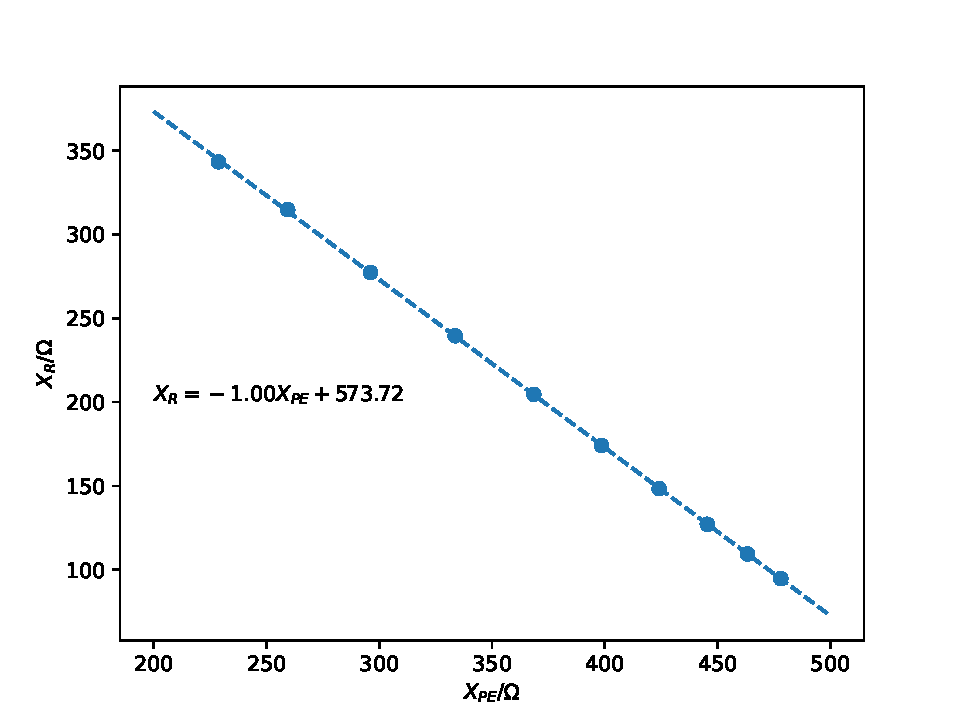
\includegraphics[width=0.7\textwidth]{fig_opt2.pdf}
    \caption{等效感抗与反射感抗关系}
    \label{fig:3}
\end{figure}
其关系为$X_R = -1.00X_{PE}+573.72\Omega$,而$573.72\Omega$恰好与线圈一的感抗十分接近,可以猜测$X_R + X = X_{PE}$。这在物理上也很合理,即等效感抗等于本身的感抗加上另一个线圈的反射感抗,是一个很自然的物理图像。

$R_R$也会随$R_L$变化而变化,为了更史观的展示这一点,做出$R_R-R_L$图,如下图:
\begin{figure}[H]
    \centering
    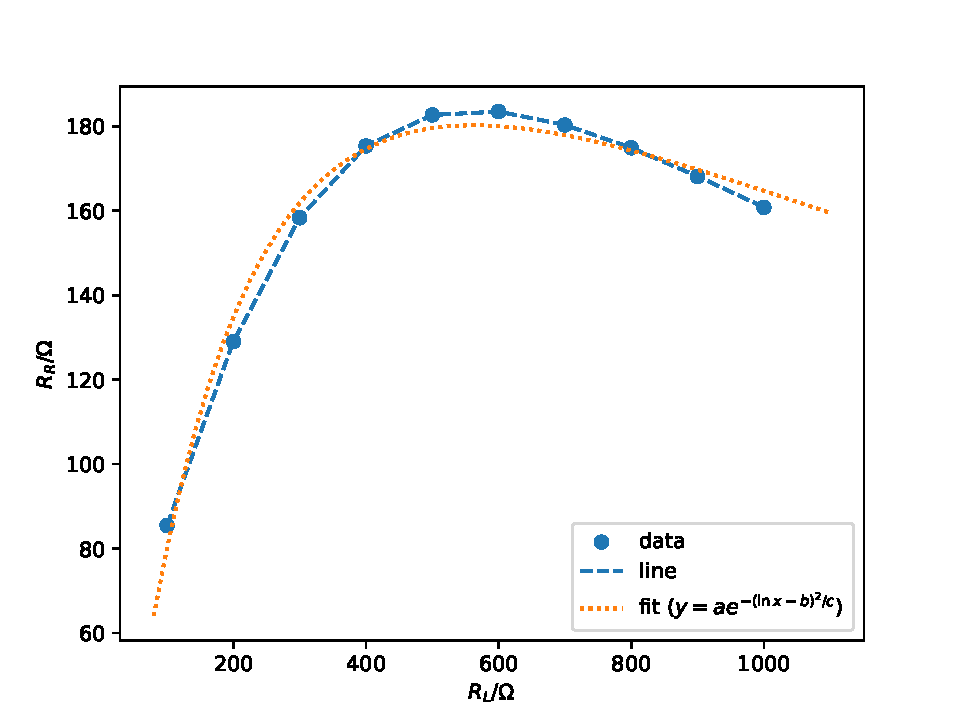
\includegraphics[width=0.7\textwidth]{fig_opt3.pdf}
    \caption{$R_R-R_L$图}
    \label{fig:4}
\end{figure}
这里,由散点图观察到是一个偏态峰,按照把偏态数据拉回正态的思路,在标准正态分布中取$\ln{x}$近似得到一个偏态拟合。由拟合及正态分布知,当$\ln{x}=b$时,$y$最大,即当反射电阻最大时,$R_L=562.3\Omega$。

\section{涡流效应}
当带电线圈中放入铝芯后,铝芯上产生的涡流使线圈感受到的电感和电阻发生改变。先求$L_{Al}$和$R_{Al}$的比值。第一部分实际上测出了等效值,故只需$\frac{L_{Al}}{R_{Al}}=|\frac{\Delta L}{\Delta R}|$,带入,对于线圈1,$\frac{L_{Al}}{R_{Al}}=3.010\times10^{-3}$;对于线圈2,$\frac{L_{Al}}{R_{Al}}=3.073\times10^{-3}$。

涡流还会造成铝芯功率损耗。我们在第二部分的基础上插入铝芯,再次测量,得到的结果如\ref{tab:A3}。根据$\Delta P = I_P^2R_{PE}-I_P^2R_P-I_S^2(R_S+R_L)$,带入数据,有$\Delta P = -1.524\times10^{-3}J$

\section{讨论}
测量时,由于接头松动,移动接头将会导致不稳定,下分析这一不稳定对结果产生的影响。

对于部分二,我还测出了频繁插拔接头的另一组数据。测量时,仪器并不能有一个稳定的读数(处于周期震荡的状态),采用肉眼目测取平均的方式来获得大致读数。用相同的方式拟合,如图:
\begin{figure}[H]
    \centering
    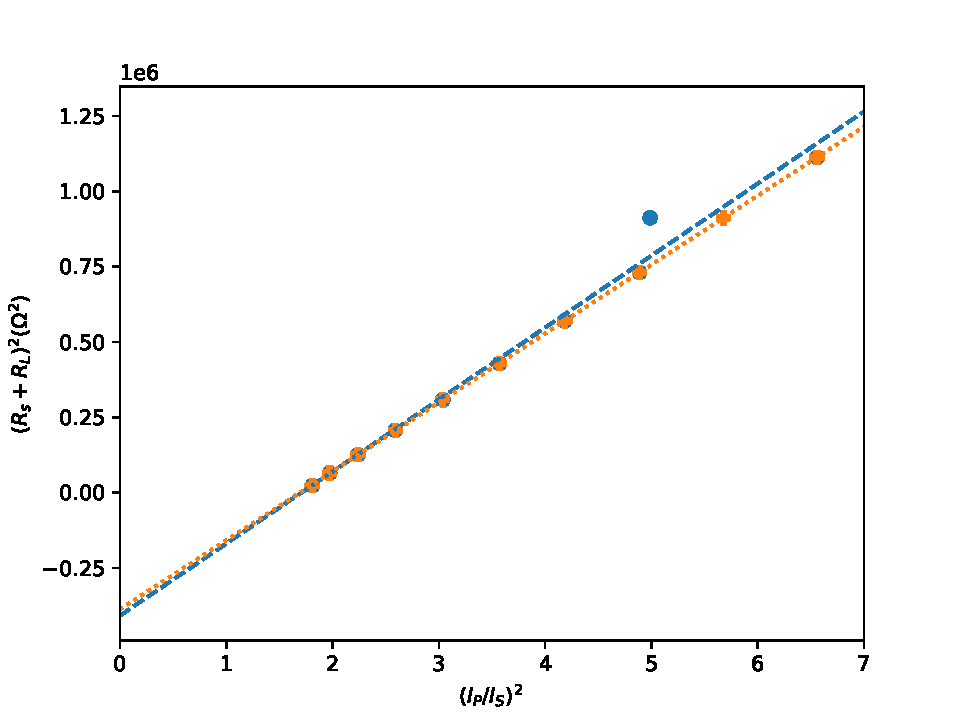
\includegraphics[width=0.7\textwidth]{fig_old.pdf}
    \caption{稳定与不稳定}
    \label{fig:5}
\end{figure}
黄色点的测量方法避免了频繁插拔,而蓝色点存在频繁插拔。可见蓝色存在一个明显离群的数据,存在较大误差。但是,如果排除该离群数据,误差其实是很小的。(甚至很多蓝/黄色点几乎重合)从这个角度看,仪器读数不稳定造成的误差微乎其微,只需要用肉眼取平均就能很容易修正。虽然交流电对这样的松动比较敏感,但实际上仪器还是比较好的连接好了。(虽然存在松动)

\clearpage
\appendix
\section{附录}
\renewcommand{\thetable}{附表\arabic{table}}
\setcounter{table}{0}
\begin{table}[H]
    \centering
    \begin{tabular}{|l|c|c|c|c|c|}
        \hline
                          & $R' (\Omega)$ & $V_A (V)$ & $V (V)$ & $V_{R'} (V)$ & $V_O (V)$ \\ \hline
        a) 测线圈1,无铝芯       & 560    & 6.753  & 4.629 & 4.512   & 3.836  \\ \hline
        c) 测线圈1,放入铝芯(有铝芯) & 470    & 6.694  & 4.386 & 4.322   & 3.000  \\ \hline
        b) 测线圈2,取下铝芯(无铝芯) & 630    & 6.778  & 4.570 & 4.621   & 3.492  \\ \hline
        d) 测线圈2,放入铝芯(有铝芯) & 410    & 6.641  & 4.100 & 4.088   & 3.250  \\ \hline
        \end{tabular}
    \caption{第一部分测量数据}
    \label{tab:A1}
\end{table}

\begin{table}[H]
    \centering
    \begin{tabular}{|c|c|c|c|c|c|}
    \hline
    $R_L(\Omega)$ & $R'(\Omega)$ & $V_A(V)$ & $V(V)$ & $V_{R'}(V)$ & $V_{R_L}(V)$ \\ \hline
    100           & 300          & 6.457    & 3.486  & 3.932       & 0.974        \\ \hline
    200           & 300          & 6.516    & 3.756  & 3.576       & 1.697        \\ \hline
    300           & 300          & 6.561    & 4.035  & 3.339       & 2.231        \\ \hline
    400           & 300          & 6.597    & 4.260  & 3.169       & 2.625        \\ \hline
    500           & 300          & 6.624    & 4.456  & 3.064       & 2.930        \\ \hline
    600           & 300          & 6.646    & 4.605  & 2.987       & 3.162        \\ \hline
    700           & 300          & 6.663    & 4.723  & 2.931       & 3.343        \\ \hline
    800           & 300          & 6.676    & 4.758  & 2.854       & 3.442        \\ \hline
    900           & 300          & 6.687    & 4.900  & 2.685       & 3.607        \\ \hline
    1000          & 300          & 6.696    & 4.972  & 2.848       & 3.707        \\ \hline
    \end{tabular}
    \caption{第二部分测量数据}
    \label{tab:A2}
\end{table}

\begin{table}[H]
    \centering
    \begin{tabular}{|c|c|c|c|c|c|}
    \hline
    $R_L (\Omega)$ & $R' (\Omega)$ & $V_A (V)$ & $V (V)$ & $V_{R'} (V)$ & $V_O (V)$ \\ \hline
    1000           & 300           & 6.645     & 4.779   & 3.221        & 2.94      \\ \hline
    \end{tabular}
    \caption{第四部分测量数据}
    \label{tab:A3}
\end{table}

所有相关文件可通过\href{https://cloud.tsinghua.edu.cn/d/8cefbd2d2132481b8647/}{清华云盘}获得。

\clearpage
课堂上数据记录表如下:(似乎没必要,看前面的表就行)
\begin{figure}[H]
    \centering
    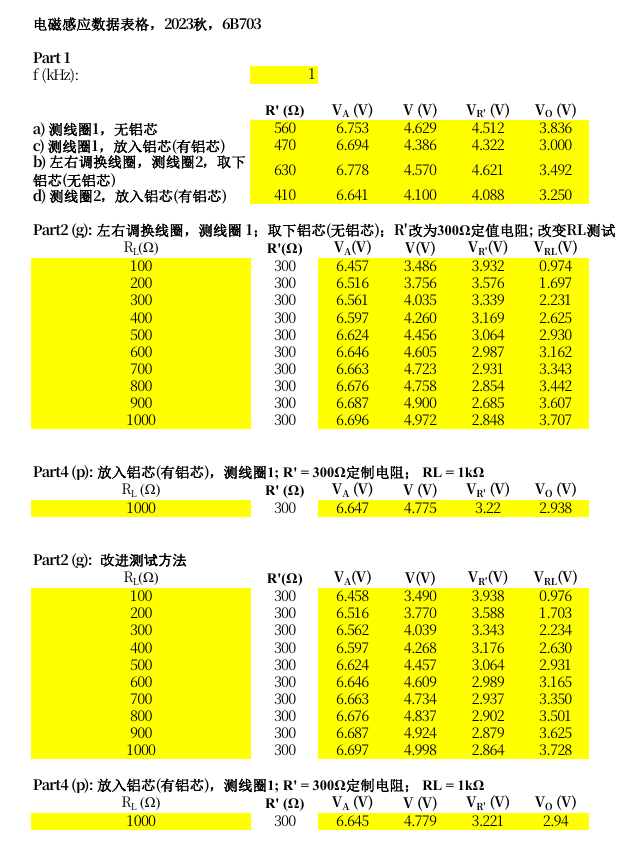
\includegraphics{Screenshot.png}
\end{figure}
\end{document}
